% Created by tikzDevice version 0.10.1 on 2018-06-27 15:24:37
% !TEX encoding = UTF-8 Unicode
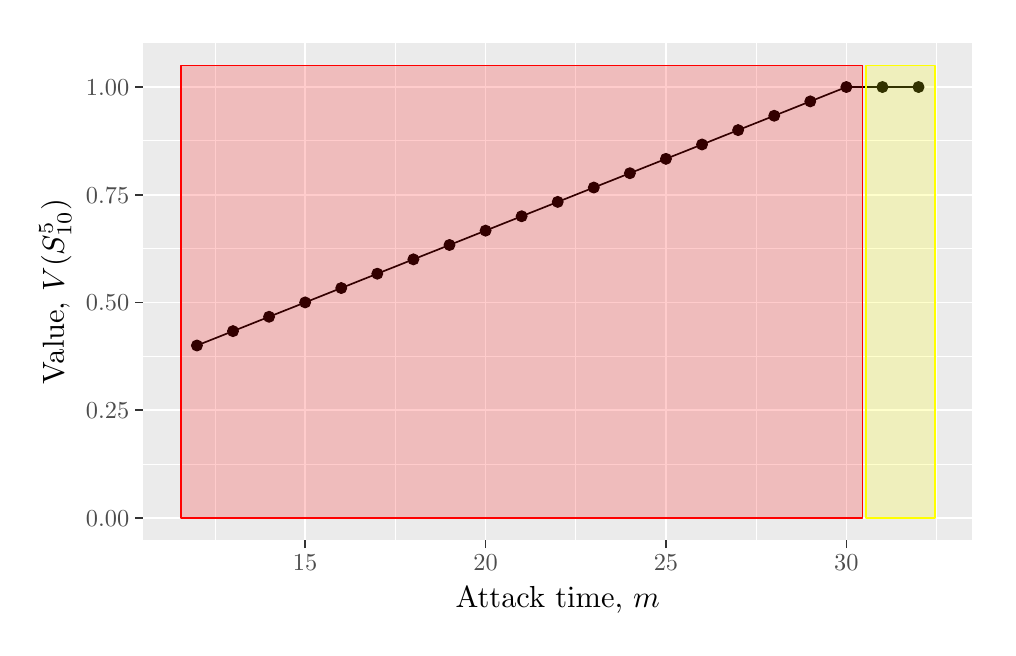
\begin{tikzpicture}[x=1pt,y=1pt]
\definecolor{fillColor}{RGB}{255,255,255}
\path[use as bounding box,fill=fillColor,fill opacity=0.00] (0,0) rectangle (346.90,216.81);
\begin{scope}
\path[clip] (  0.00,  0.00) rectangle (346.90,216.81);
\definecolor{drawColor}{RGB}{255,255,255}
\definecolor{fillColor}{RGB}{255,255,255}

\path[draw=drawColor,line width= 0.6pt,line join=round,line cap=round,fill=fillColor] (  0.00,  0.00) rectangle (346.90,216.81);
\end{scope}
\begin{scope}
\path[clip] ( 41.67, 31.53) rectangle (341.40,211.31);
\definecolor{fillColor}{gray}{0.92}

\path[fill=fillColor] ( 41.67, 31.53) rectangle (341.40,211.31);
\definecolor{drawColor}{RGB}{255,255,255}

\path[draw=drawColor,line width= 0.3pt,line join=round] ( 41.67, 59.16) --
	(341.40, 59.16);

\path[draw=drawColor,line width= 0.3pt,line join=round] ( 41.67, 98.07) --
	(341.40, 98.07);

\path[draw=drawColor,line width= 0.3pt,line join=round] ( 41.67,136.99) --
	(341.40,136.99);

\path[draw=drawColor,line width= 0.3pt,line join=round] ( 41.67,175.90) --
	(341.40,175.90);

\path[draw=drawColor,line width= 0.3pt,line join=round] ( 67.68, 31.53) --
	( 67.68,211.31);

\path[draw=drawColor,line width= 0.3pt,line join=round] (132.86, 31.53) --
	(132.86,211.31);

\path[draw=drawColor,line width= 0.3pt,line join=round] (198.05, 31.53) --
	(198.05,211.31);

\path[draw=drawColor,line width= 0.3pt,line join=round] (263.24, 31.53) --
	(263.24,211.31);

\path[draw=drawColor,line width= 0.3pt,line join=round] (328.42, 31.53) --
	(328.42,211.31);

\path[draw=drawColor,line width= 0.6pt,line join=round] ( 41.67, 39.70) --
	(341.40, 39.70);

\path[draw=drawColor,line width= 0.6pt,line join=round] ( 41.67, 78.62) --
	(341.40, 78.62);

\path[draw=drawColor,line width= 0.6pt,line join=round] ( 41.67,117.53) --
	(341.40,117.53);

\path[draw=drawColor,line width= 0.6pt,line join=round] ( 41.67,156.44) --
	(341.40,156.44);

\path[draw=drawColor,line width= 0.6pt,line join=round] ( 41.67,195.36) --
	(341.40,195.36);

\path[draw=drawColor,line width= 0.6pt,line join=round] (100.27, 31.53) --
	(100.27,211.31);

\path[draw=drawColor,line width= 0.6pt,line join=round] (165.46, 31.53) --
	(165.46,211.31);

\path[draw=drawColor,line width= 0.6pt,line join=round] (230.64, 31.53) --
	(230.64,211.31);

\path[draw=drawColor,line width= 0.6pt,line join=round] (295.83, 31.53) --
	(295.83,211.31);
\definecolor{drawColor}{RGB}{0,0,0}
\definecolor{fillColor}{RGB}{0,0,0}

\path[draw=drawColor,line width= 0.4pt,line join=round,line cap=round,fill=fillColor] (308.87,195.36) circle (  1.96);

\path[draw=drawColor,line width= 0.4pt,line join=round,line cap=round,fill=fillColor] (321.91,195.36) circle (  1.96);

\path[draw=drawColor,line width= 0.4pt,line join=round,line cap=round,fill=fillColor] ( 61.16,101.96) circle (  1.96);

\path[draw=drawColor,line width= 0.4pt,line join=round,line cap=round,fill=fillColor] ( 74.19,107.15) circle (  1.96);

\path[draw=drawColor,line width= 0.4pt,line join=round,line cap=round,fill=fillColor] ( 87.23,112.34) circle (  1.96);

\path[draw=drawColor,line width= 0.4pt,line join=round,line cap=round,fill=fillColor] (100.27,117.53) circle (  1.96);

\path[draw=drawColor,line width= 0.4pt,line join=round,line cap=round,fill=fillColor] (113.31,122.72) circle (  1.96);

\path[draw=drawColor,line width= 0.4pt,line join=round,line cap=round,fill=fillColor] (126.34,127.91) circle (  1.96);

\path[draw=drawColor,line width= 0.4pt,line join=round,line cap=round,fill=fillColor] (139.38,133.09) circle (  1.96);

\path[draw=drawColor,line width= 0.4pt,line join=round,line cap=round,fill=fillColor] (152.42,138.28) circle (  1.96);

\path[draw=drawColor,line width= 0.4pt,line join=round,line cap=round,fill=fillColor] (165.46,143.47) circle (  1.96);

\path[draw=drawColor,line width= 0.4pt,line join=round,line cap=round,fill=fillColor] (178.49,148.66) circle (  1.96);

\path[draw=drawColor,line width= 0.4pt,line join=round,line cap=round,fill=fillColor] (191.53,153.85) circle (  1.96);

\path[draw=drawColor,line width= 0.4pt,line join=round,line cap=round,fill=fillColor] (204.57,159.04) circle (  1.96);

\path[draw=drawColor,line width= 0.4pt,line join=round,line cap=round,fill=fillColor] (217.61,164.22) circle (  1.96);

\path[draw=drawColor,line width= 0.4pt,line join=round,line cap=round,fill=fillColor] (230.64,169.41) circle (  1.96);

\path[draw=drawColor,line width= 0.4pt,line join=round,line cap=round,fill=fillColor] (243.68,174.60) circle (  1.96);

\path[draw=drawColor,line width= 0.4pt,line join=round,line cap=round,fill=fillColor] (256.72,179.79) circle (  1.96);

\path[draw=drawColor,line width= 0.4pt,line join=round,line cap=round,fill=fillColor] (269.76,184.98) circle (  1.96);

\path[draw=drawColor,line width= 0.4pt,line join=round,line cap=round,fill=fillColor] (282.79,190.17) circle (  1.96);

\path[draw=drawColor,line width= 0.4pt,line join=round,line cap=round,fill=fillColor] (295.83,195.36) circle (  1.96);

\path[draw=drawColor,line width= 0.6pt,line join=round] ( 61.16,101.96) --
	( 74.19,107.15) --
	( 87.23,112.34) --
	(100.27,117.53) --
	(113.31,122.72) --
	(126.34,127.91) --
	(139.38,133.09) --
	(152.42,138.28) --
	(165.46,143.47) --
	(178.49,148.66) --
	(191.53,153.85) --
	(204.57,159.04) --
	(217.61,164.22) --
	(230.64,169.41) --
	(243.68,174.60) --
	(256.72,179.79) --
	(269.76,184.98) --
	(282.79,190.17) --
	(295.83,195.36) --
	(308.87,195.36) --
	(321.91,195.36);
\definecolor{drawColor}{RGB}{255,255,0}
\definecolor{fillColor}{RGB}{255,255,0}

\path[draw=drawColor,line width= 0.6pt,line join=round,fill=fillColor,fill opacity=0.20] (303.00, 39.70) rectangle (327.77,203.14);
\definecolor{drawColor}{RGB}{255,0,0}
\definecolor{fillColor}{RGB}{255,0,0}

\path[draw=drawColor,line width= 0.6pt,line join=round,fill=fillColor,fill opacity=0.20] ( 55.29, 39.70) rectangle (301.70,203.14);
\end{scope}
\begin{scope}
\path[clip] (  0.00,  0.00) rectangle (346.90,216.81);
\definecolor{drawColor}{gray}{0.30}

\node[text=drawColor,anchor=base east,inner sep=0pt, outer sep=0pt, scale=  0.88] at ( 36.72, 36.67) {0.00};

\node[text=drawColor,anchor=base east,inner sep=0pt, outer sep=0pt, scale=  0.88] at ( 36.72, 75.59) {0.25};

\node[text=drawColor,anchor=base east,inner sep=0pt, outer sep=0pt, scale=  0.88] at ( 36.72,114.50) {0.50};

\node[text=drawColor,anchor=base east,inner sep=0pt, outer sep=0pt, scale=  0.88] at ( 36.72,153.41) {0.75};

\node[text=drawColor,anchor=base east,inner sep=0pt, outer sep=0pt, scale=  0.88] at ( 36.72,192.33) {1.00};
\end{scope}
\begin{scope}
\path[clip] (  0.00,  0.00) rectangle (346.90,216.81);
\definecolor{drawColor}{gray}{0.20}

\path[draw=drawColor,line width= 0.6pt,line join=round] ( 38.92, 39.70) --
	( 41.67, 39.70);

\path[draw=drawColor,line width= 0.6pt,line join=round] ( 38.92, 78.62) --
	( 41.67, 78.62);

\path[draw=drawColor,line width= 0.6pt,line join=round] ( 38.92,117.53) --
	( 41.67,117.53);

\path[draw=drawColor,line width= 0.6pt,line join=round] ( 38.92,156.44) --
	( 41.67,156.44);

\path[draw=drawColor,line width= 0.6pt,line join=round] ( 38.92,195.36) --
	( 41.67,195.36);
\end{scope}
\begin{scope}
\path[clip] (  0.00,  0.00) rectangle (346.90,216.81);
\definecolor{drawColor}{gray}{0.20}

\path[draw=drawColor,line width= 0.6pt,line join=round] (100.27, 28.78) --
	(100.27, 31.53);

\path[draw=drawColor,line width= 0.6pt,line join=round] (165.46, 28.78) --
	(165.46, 31.53);

\path[draw=drawColor,line width= 0.6pt,line join=round] (230.64, 28.78) --
	(230.64, 31.53);

\path[draw=drawColor,line width= 0.6pt,line join=round] (295.83, 28.78) --
	(295.83, 31.53);
\end{scope}
\begin{scope}
\path[clip] (  0.00,  0.00) rectangle (346.90,216.81);
\definecolor{drawColor}{gray}{0.30}

\node[text=drawColor,anchor=base,inner sep=0pt, outer sep=0pt, scale=  0.88] at (100.27, 20.52) {15};

\node[text=drawColor,anchor=base,inner sep=0pt, outer sep=0pt, scale=  0.88] at (165.46, 20.52) {20};

\node[text=drawColor,anchor=base,inner sep=0pt, outer sep=0pt, scale=  0.88] at (230.64, 20.52) {25};

\node[text=drawColor,anchor=base,inner sep=0pt, outer sep=0pt, scale=  0.88] at (295.83, 20.52) {30};
\end{scope}
\begin{scope}
\path[clip] (  0.00,  0.00) rectangle (346.90,216.81);
\definecolor{drawColor}{RGB}{0,0,0}

\node[text=drawColor,anchor=base,inner sep=0pt, outer sep=0pt, scale=  1.10] at (191.53,  7.44) {Attack time, $m$};
\end{scope}
\begin{scope}
\path[clip] (  0.00,  0.00) rectangle (346.90,216.81);
\definecolor{drawColor}{RGB}{0,0,0}

\node[text=drawColor,rotate= 90.00,anchor=base,inner sep=0pt, outer sep=0pt, scale=  1.10] at ( 13.08,121.42) {Value, $V(S_{ 10 }^{ 5 })$};
\end{scope}
\end{tikzpicture}
